\documentclass[uft8]{article}
\usepackage{amsmath}
\usepackage{graphicx}
\usepackage{longtable}

\begin{document}
$\kappa$ = 0.74

Degree = 1

Method = Boundary Integral Operators

FMM Order = 10

\begin{longtable}{c c}
d.o.f. Count & Relative Error \\ \hline
80 & 7.72e-02 \\ \hline
212 & 2.89e-02 \\ \hline
736 & 1.94e-02 \\ \hline
2963 & 2.85e-03 \\ \hline
11261 & 8.62e-04 \\ \hline
44627 & 2.13e-04 \\ \hline
178882 & 7.66e-05 \\ \hline
\end{longtable}

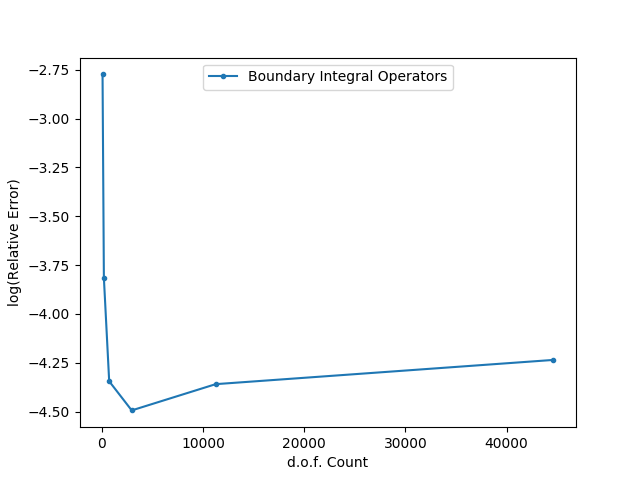
\includegraphics[width=\textwidth]{fig--free--ongraph_method-coupling--req--x_ndof--y_rel_err.png}\\ 


\end{document}
